\chapter{Scénario}\label{scenario}

\section{Textes}

Le jeu ne contient que deux phrases qui seront affichées à l'écran :
\begin{itemize}
  \item \textit{Trouvez la sortie} : affiché au tout début du jeu.
  \item \textit{Bravo ! Vous avez trouvé la sortie !} : affiché en fin de jeu, lorsque l'utilisateur parvient à trouver la sortie.
\end{itemize}

\begin{figure}[h!]
  \centering
  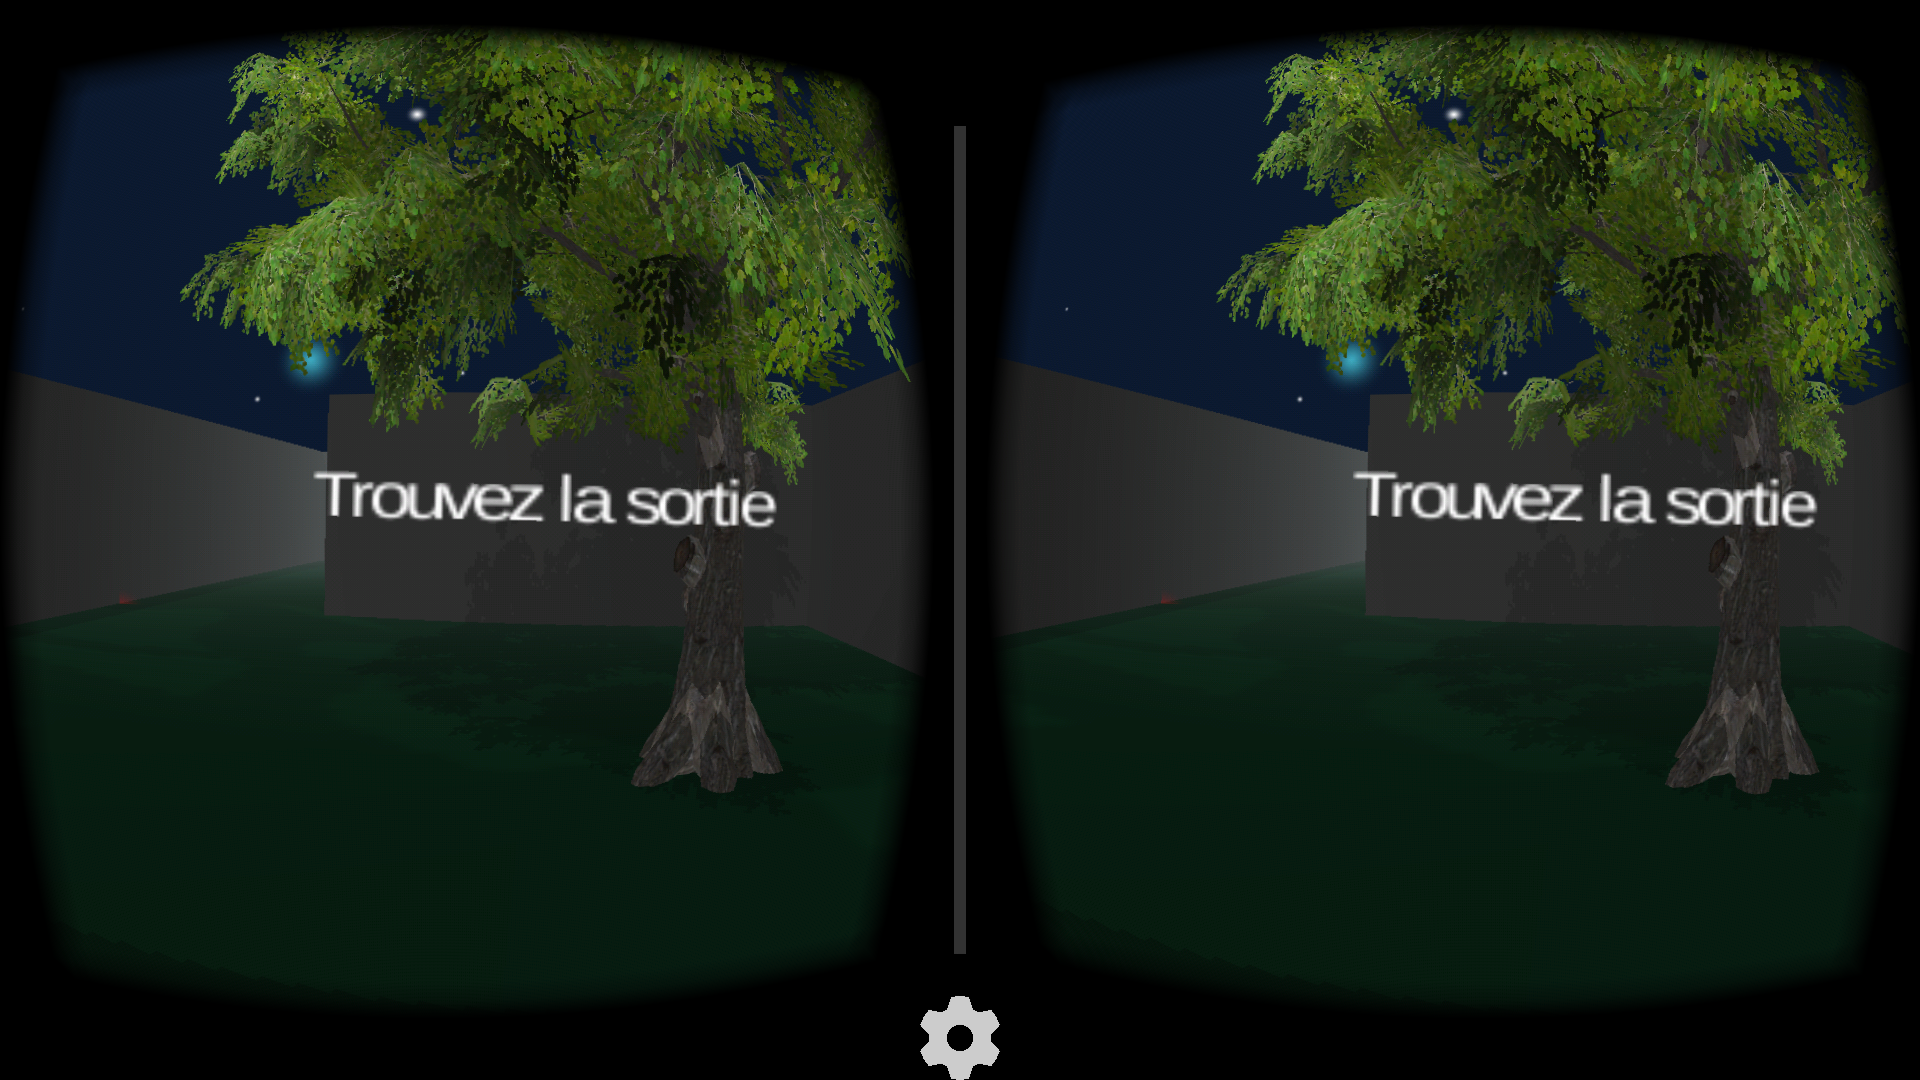
\includegraphics[width=1.0\textwidth]{res/img/trouvez-la-sortie.png}
  \caption{Démarrage du jeu}
\end{figure}

\section{Mise en scène}
Au lancement de l'application Android, le joueur est directement placé au c\oe{}ur du labyrinthe, près d'un grand arbre et son seul but est d'en sortir. Pour cela, il s'oriente vers la gauche et la droite pour tourner, tandis que son personnage fictif est à l'arrêt. La musique de fond commence immédiatement. Une action sur le bouton des Cardboard (l'aimant) permet de commencer à avancer : le joueur se déplace alors vers l'avant. Il doit donc maintenant s'orienter et parvenir à sortir du labyrinthe. Son seul répère visuel dans l'immensité du lbayrinthe est le grand arbre du début, que l'on peut apercevoir de partout.

\medskip

Des particules lumineuses volantes ainsi que du vent (qui fait mouvoir des éléments du décor, comme un arbre ou un buisson) viennent dynamiser l'environnement.

\begin{figure}[h!]
  \centering
  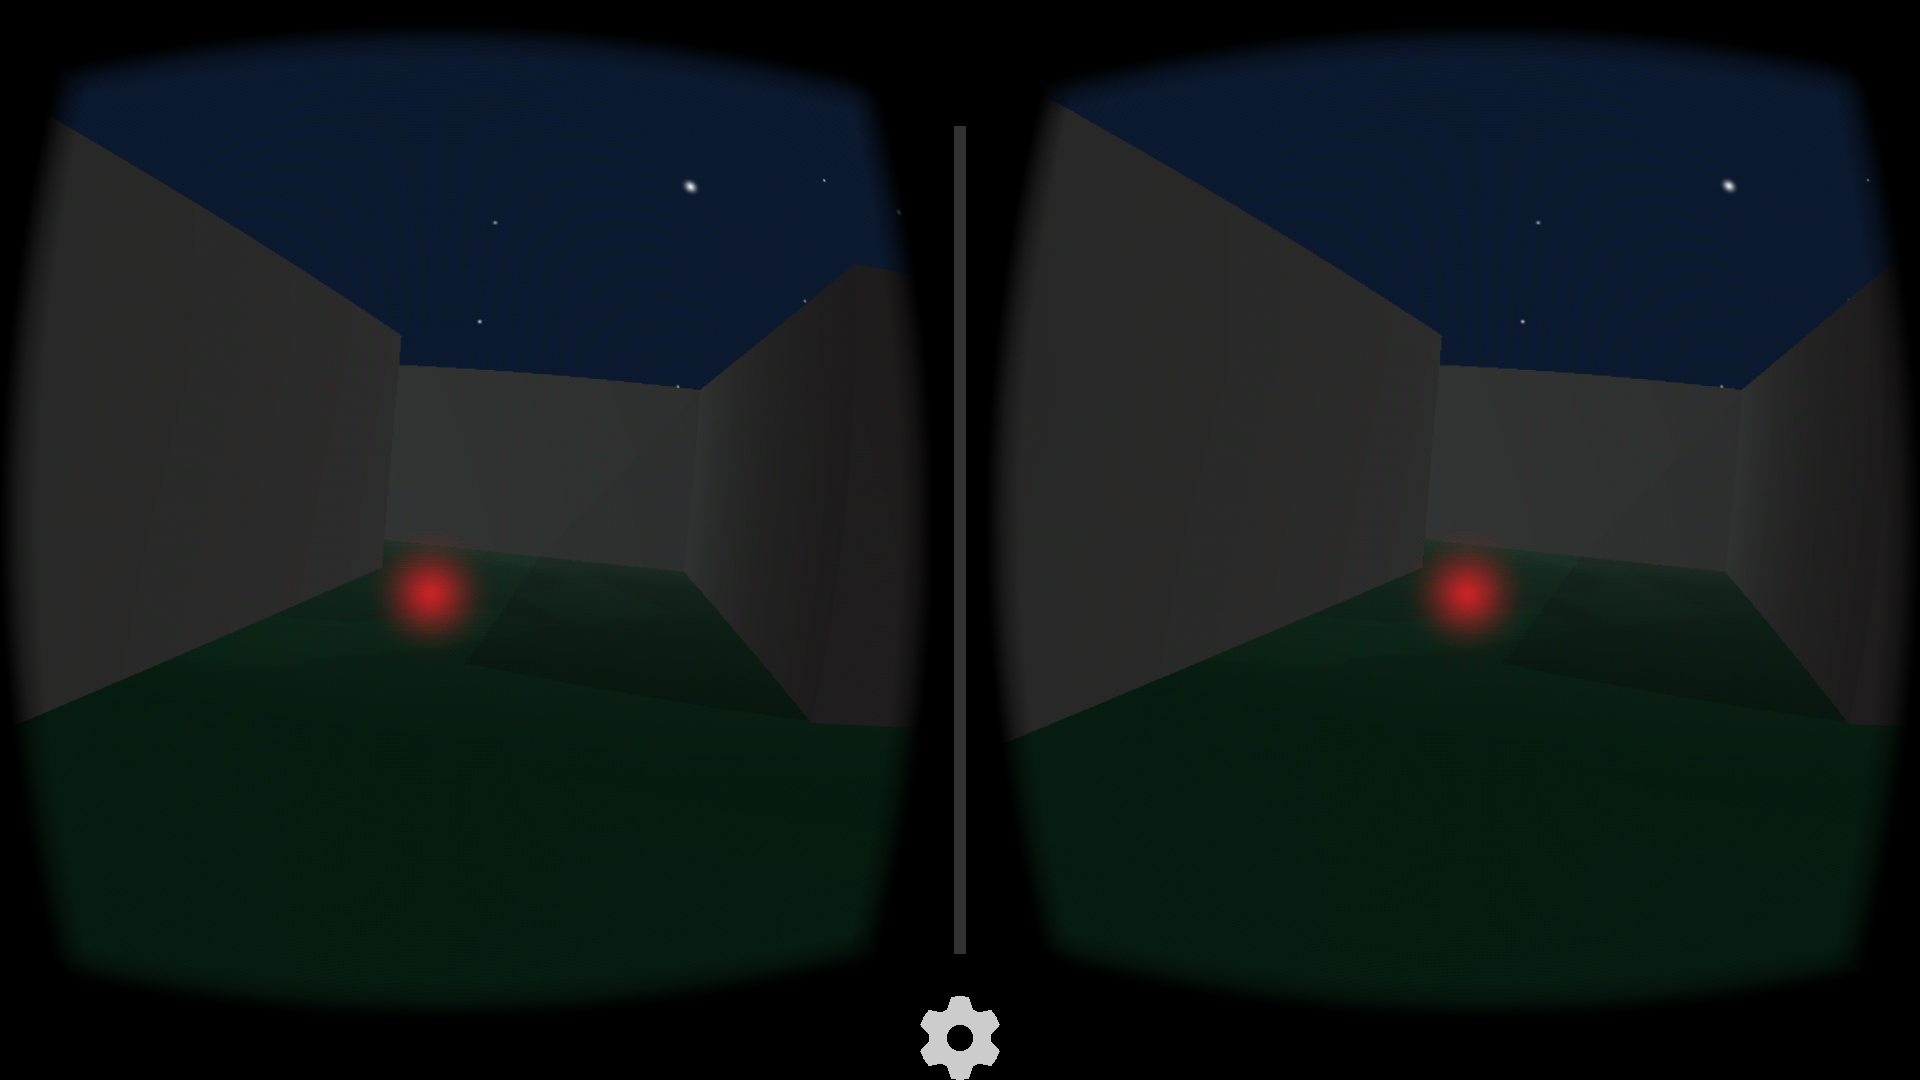
\includegraphics[width=1.0\textwidth]{res/img/couloir.png}
  \caption{Un couloir du jeu, avec des particules lumineuses volantes}
\end{figure}
